\chapter{Determining the presence of NLOS component}

The first set of practical measurements was carried out in order to determine the presence and observe the characteristics of the non-line-of-sight component of the signal. 

\section{Measurements setup}
\label{sec:Test1_meas_scenario}

The measurements were obtained using Nokia's sensing proof-of-concept described in section \ref{sec:intro-PoCarchitecture}. The system was mounted in an indoor industrial test facility, with gNB and sniffer positioned at a height of $5,12$ m. The transmitter was oriented towards a wide  indoor area free of obstacles. The antenna pole was located approximately 23 metres away from a warehouse rack (which was in front of a wall) and a cargo door.

The measurement area observed was free of any major obstructions or occlusions that could be used to create a non-line-of-sight scenario under normal conditions. 
 


The tests were carried out using:

\begin{enumerate}
	\item A human target.
	\item A strong reflector (large metal cabinet with flat surfaces).
\end{enumerate}

The direction (azimuth $\theta$ and elevation $\varphi$) of the transmitted beam was fixed for the whole measurement.

Before each test, a short calibration measure is performed, which includes only the static elements of the scenario. The calibration data will be used in the post-processing steps for subspace-based clutter removal with the \textit{CRAP} method  \cite{Henninger_CRAP_2023}. 

\alert{TODO: NOW SHOW NEW MEAS USING ECA-C, COMPARE THE TWO, DISCUSS FALSE ALARMS RATES, DISCUSS POSITION OFFSET IN ECA-C}


% TODO: check if axes are needed
\begin{figure}[H]
	\centering
	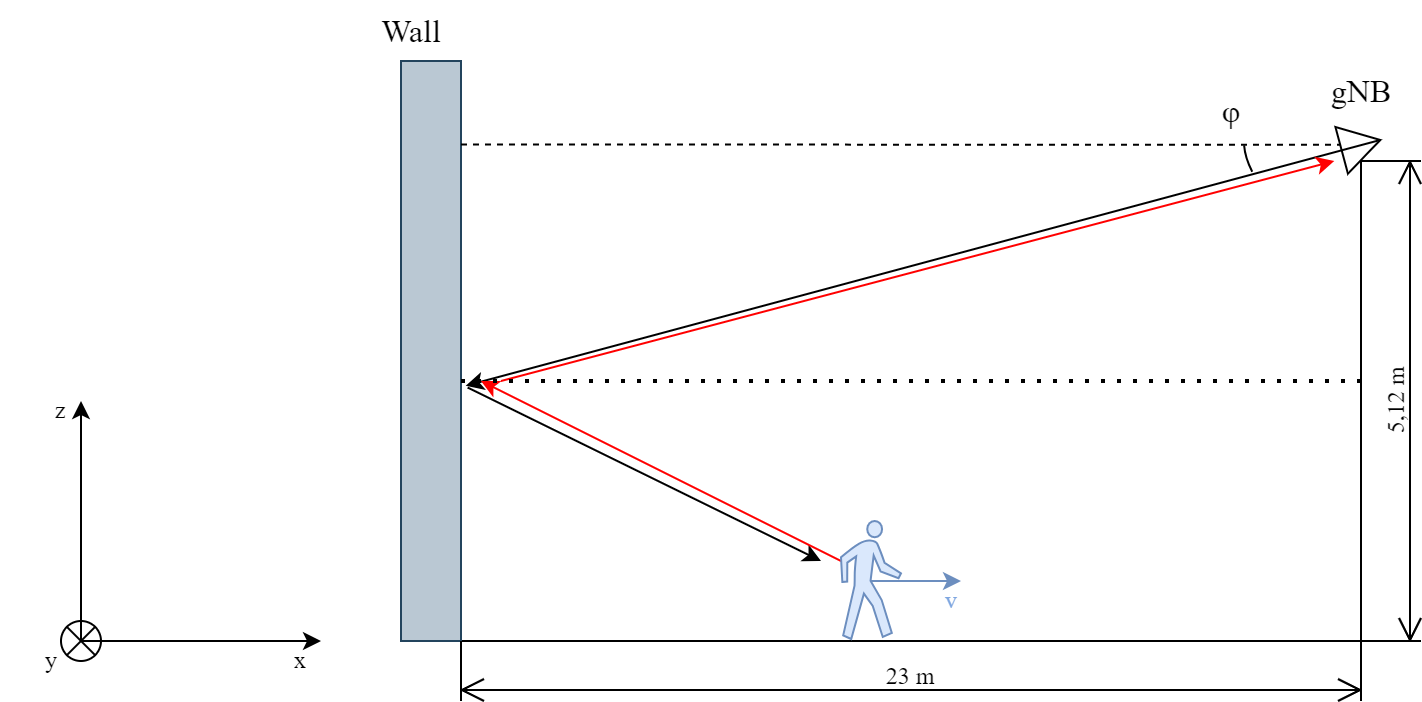
\includegraphics[width=1\textwidth]{Images/Test1/base-lateral_view}
	\caption{Lateral view of measurement scenario.}
	\label{fig:Test1_base-lateral_view}
\end{figure}

\section{Moving target without obstructions}

The OFDM radar system will be able to determine the range and radial speed (the angle of arrival AOA is fixed) of a target. If an object is moving azimuthally inside the transmitted beam, it will appear as static to the sensing system.

The aim of the test was to maximize the radial speed for the target under test, in order to analyze the characteristics of the signal generated from its reflection.

During the initial measurement the antenna boresight was directed perpendicular to the wall,while the target moved radially between the transmitter and reflector.

\begin{figure}[H]
	\centering
	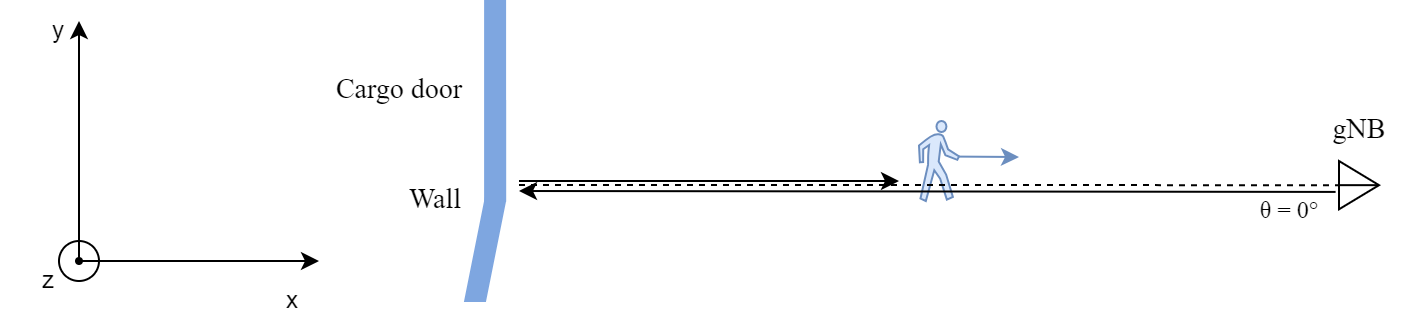
\includegraphics[width=1\textwidth]{Images/Test1/base-top_view}
	\caption{Top view of measurement scenario.}
	\label{fig:Test1_base-top_view}
\end{figure}


Beam elevation was chosen to be as high as possible in order to avoid line-of-sight from the transmitted beam's main lobe. Beam parameters are shown in table \ref{table:Test1TXBeamParams}.


% TODO: check if it's the case of adding something to the table
\begin{table}[H]
	%\caption*{\textbf{Title of Table (optional)}}
	\centering 
	\begin{tabular}{|p{9em} c c |}
		\hline
		\rowcolor{bluepoli!40} % comment this line to remove the color
		\textbf{} & \textbf{$\theta$ (azimuth [\textdegree])} & \textbf{$\varphi$ (elevation [\textdegree])} \T\B \\
		\hline \hline
		$\textbf{TX beam}$ & $\approx 0$ & $4$ \T\B \\
		
		\hline
	\end{tabular}
	\\[10pt]
	\caption{Transmitted beam parameters for initial measurements.}
	\label{table:Test1TXBeamParams}
\end{table}


\subsection{Line-of-sight and non-line-of-sight separation}

In order to process

In addition to clutter removal, calibration measurements provide valuable information for the determination of the distance threshold at which targets can be accurately classified as NLOS. A portion of the calibration frames can be processed as radar frames, with a focus on the analysis of the zero-Doppler component.
	

\begin{figure}[H]
	\centering
	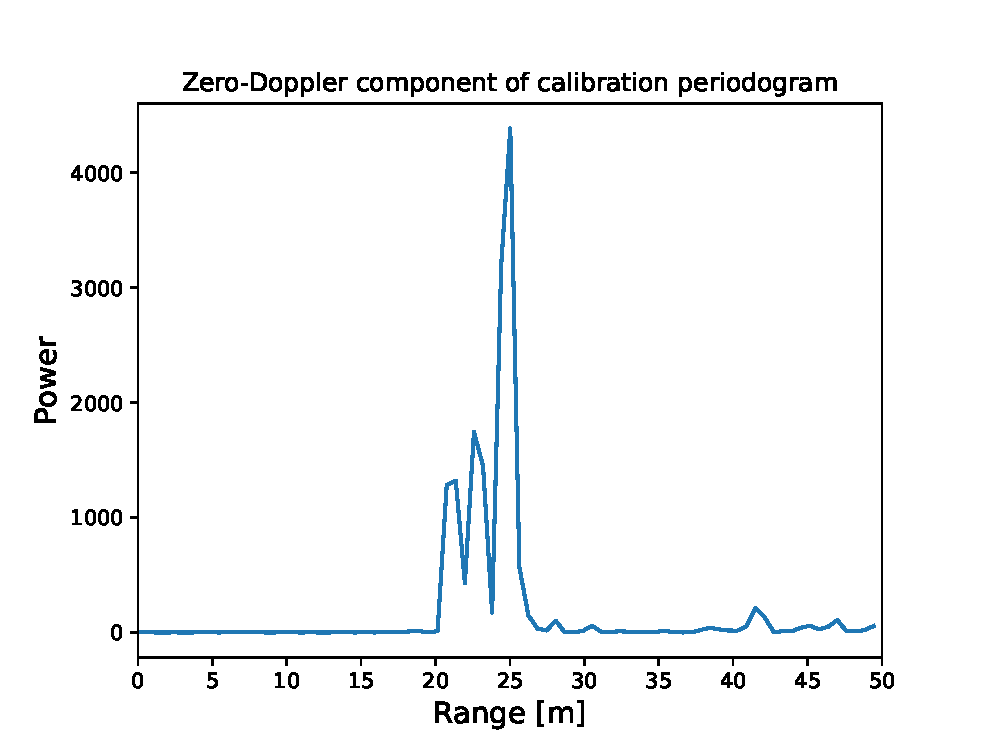
\includegraphics[width=0.6\textwidth]{Images/Test1/cali_static_per_t1.eps}
	\caption{Zero Doppler component of a periodogram generated from calibration measurements.}
	\label{fig:Test1_cali_static_per}
\end{figure}

As can be seen in the figure \ref{fig:Test1_cali_static_per}, a target with large RCS is present approximately $25$ m from the system. It was assumed that any return associated with a range greater than $25$ m was generated by a signal reflected from the main target. The figure also indicates that static clutter has a larger amplitude for ranges greater than $25$ m compared to lower ranges. This is due to the part of the beam that is reflected from the wall towards the environment and the associated returns.

The distance of the main reflector of the NLOS components was estimated by averaging the measured distance of the strongest static return from one every fifty frames during calibration.

Identifying static NLOS targets from the background was challenging due to the high power of clutter in the NLOS region, even after applying clutter removal techniques. However, it was easier to detect obscured targets by analysing the region of the periodogram associated to returns with non-zero relative speeds. The separation of the regions is highlighted in figure \ref{fig:Test1_nlos_los_separation}.

\begin{figure}[H]
	\centering
	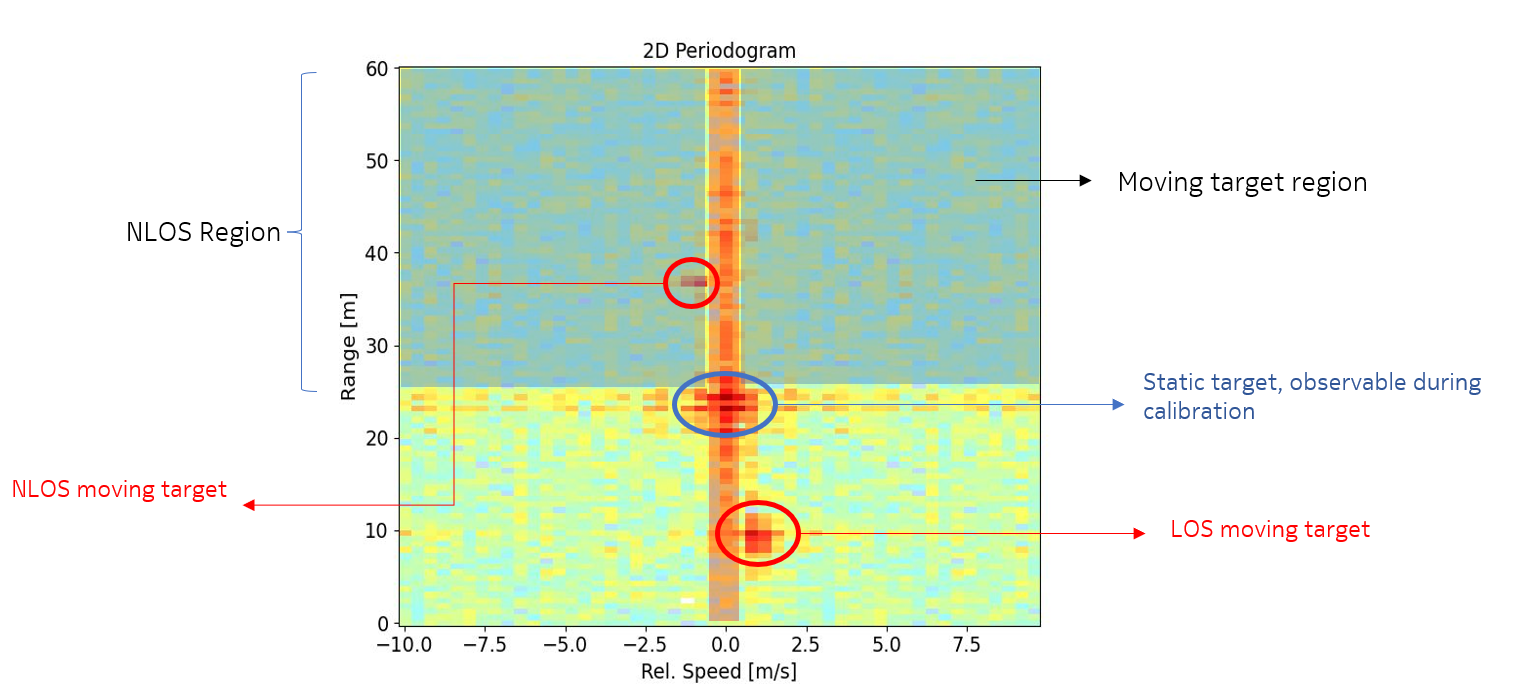
\includegraphics[width=0.9\textwidth]{Images/Test1/nlos-los-separation.png}
	\caption{Processed periodogram, separated in processing regions.}
	\label{fig:Test1_nlos_los_separation}
\end{figure}


After the periodogram has been generated, this separation can be taken into account in the post-processing phase to process the NLOS section separately from the LOS section.

\subsection{Line-of-sight component as ground truth}

Due to the rather large beamwidth of the system, $\pm$7\textdegree\hspace{1pt} in azimuth and elevation, and its sidelobes, the measurement observed the presence of a LOS target return in addition to the expected NLOS one generated by reflection.

During the measurement, the direct component was always visible as no other obstacle was positioned in the scene. It was then decided to use this component and the knowledge of the target geometry to obtain an estimate of the position and velocity of the NLOS return. This estimate was used to check if any of the detected peaks corresponded to the moving target.

\textit{Detection rate} was defined as the metric used to evaluate the experiment: if the speed and range of the NLOS return matched the expected values calculated from the LOS data detection, detection was considered positive.
The detection rate was then obtained as the ratio between the number of frames in which the NLOS component was above threshold and identified, and the total number of frames in which the LOS component was detected.

\subsection{Processing of the NLOS region}

After defining the two regions of interest from the periodogram, peak detection is conducted separately for each. A standard strongest peak search is performed for the LOS region, and accurate range and velocity measurements are obtained after interpolation of the adjacent bins.

\begin{figure}[H]
	\centering
	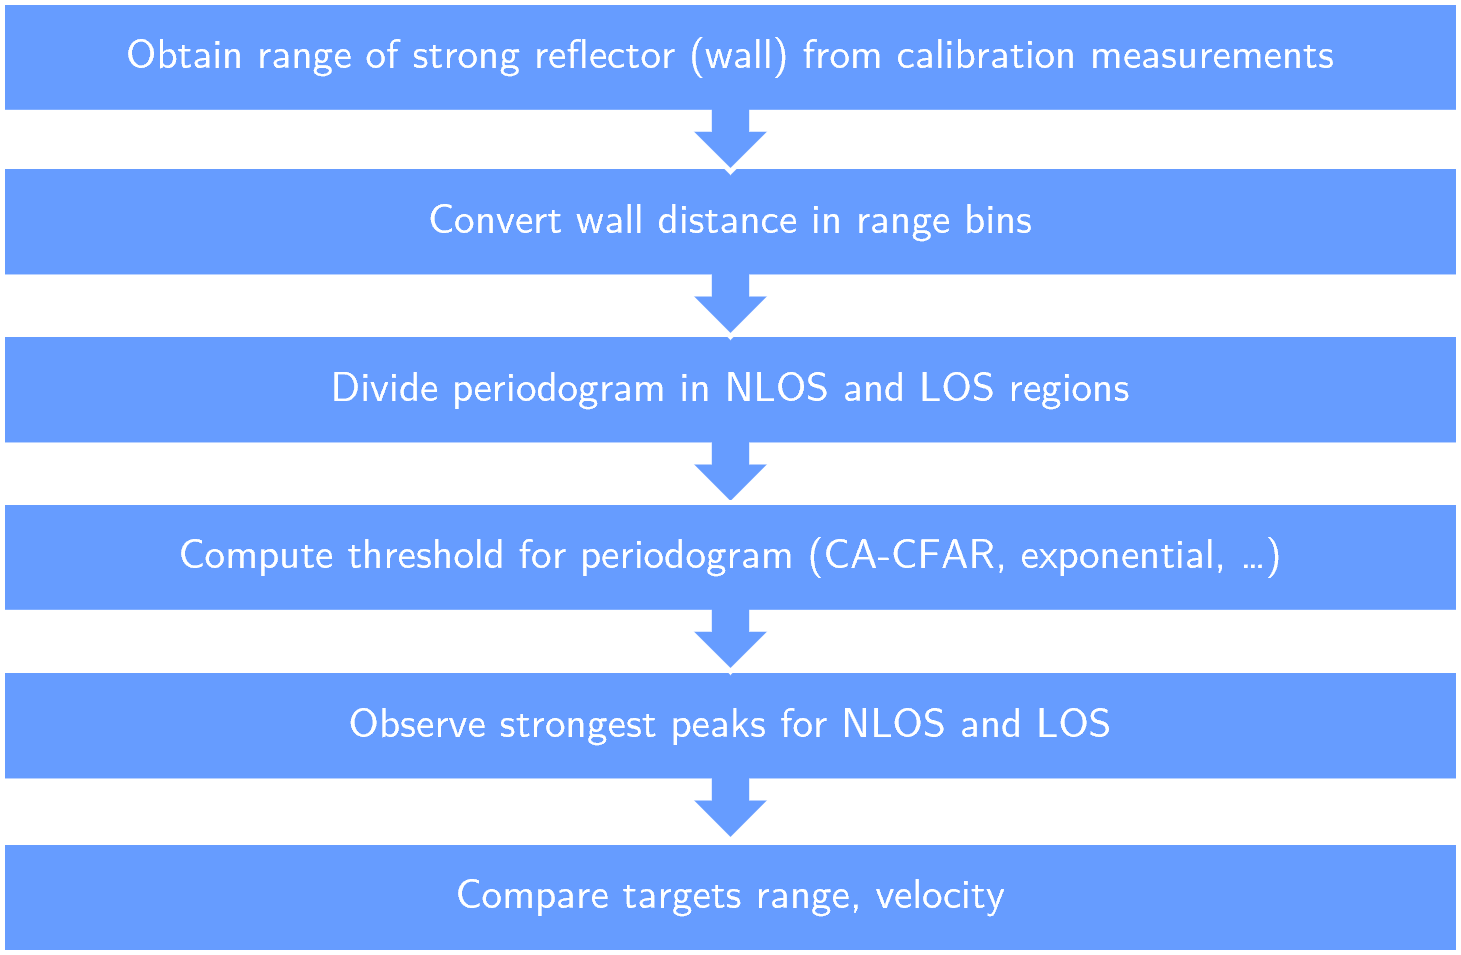
\includegraphics[width=0.9\textwidth]{Images/Test1/NLOS-proc-pipeline.png}
	\caption{Periodogram processing pipeline used for detection tests.}
	\label{fig:Test1_NLOS-proc-pipeline}
\end{figure}


Due to the presence of strong clutter components in the bins close to zero speed, the target search in the NLOS region was performed neglecting this part of the periodogram.

The full process for the experiment is summarized in figure \ref{fig:Test1_NLOS-proc-pipeline}.

The chosen detection strategy was CA-CFAR, which utilized a square contribution window and a probability of false alarm $p_{\text{FA}} = 10^{-6}$. The size of the CA-CFAR window was set depending on the width of the target in speed bins, which depended on number of processed frames and OFDM sampled symbols.
% TODO: add info on target dimensions for CA-CFAR, human case since guard cells were set in meters

\subsection{Observed detection rate}

The results were obtained with the different frame processing strategies presented in chapter \ref{chap:TDD pattern of the OFDM frame}. When combining subsequent frames to increase time-aperture, the window processing stride was set to be lower then the number of frames. This allowed to increase the amount of target updates.

Target detection was carried out considering the \textit{n}-strongest peaks and comparing them against the LOS data. If any of the observed NLOS peaks was deemed to be corresponding to the target then detection was positive.

\begin{figure}[H]
	\centering
	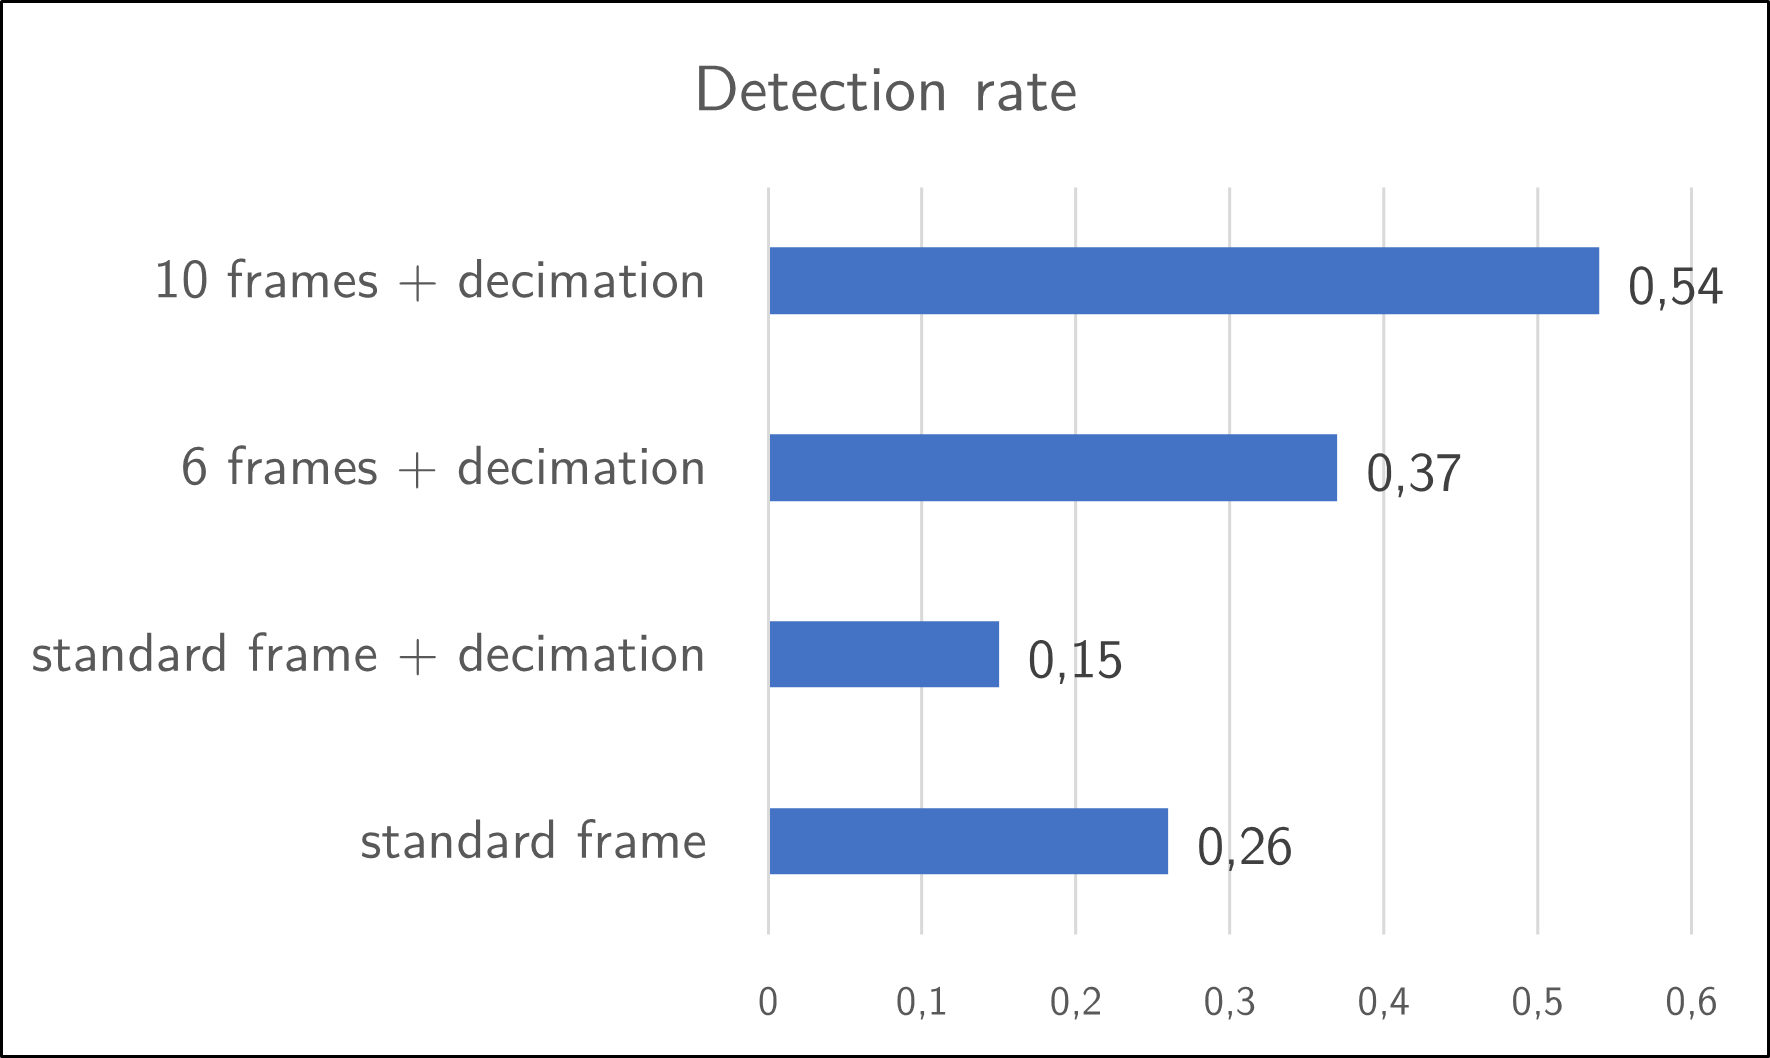
\includegraphics[width=0.7\textwidth]{Images/Test1/detect_hist.png}
	\caption{Detection rate observed for human target in mixed LOS/NLOS measurement.}
	\label{fig:Test1_detect_hist}
\end{figure}

Using a larger time-aperture significantly increased the detection rate due to the improved speed resolution. However, this approach may cause range spreading issues, particularly for fast targets. This phenomenon is not a significant drawback in NLOS sensing since the system's primary objective is target detection rather than precise tracking and positioning.

It was observed that the NLOS target return was not the strongest return in the majority of cases, with lower peak power with respect to noise and spectral artefacts, also due to channel fading.

The detection rate was observed over the whole measurement: frames in which the target changed direction and was therefore static, or presented a low speed component, were included. Processing these time instants meant that the NLOS component was likely to be masked by clutter and give a negative detection. The effective detection rate, measured only when the target is moving, is likely to be higher.

%TODO: change subsection title
\subsubsection{Moving average of detection rate}


% TODO: I don't like this phrasing
The average detection rate over 10 consecutive updates is shown in figure \ref{fig:Test1_moving_avg}. It can be seen that when the target is moving, and therefore  well separated from the clutter region, detection rate appears to be above 80\% for a number of consecutive 10-update intervals.

Although obtained in a controlled single target scenario, this measure opens the door to the possibility of determining the presence of NLOS moving targets without the aid of ground truth data.


% TODO: change picture with higher resolution one, maybe solved
\begin{figure}[H]
	\centering
	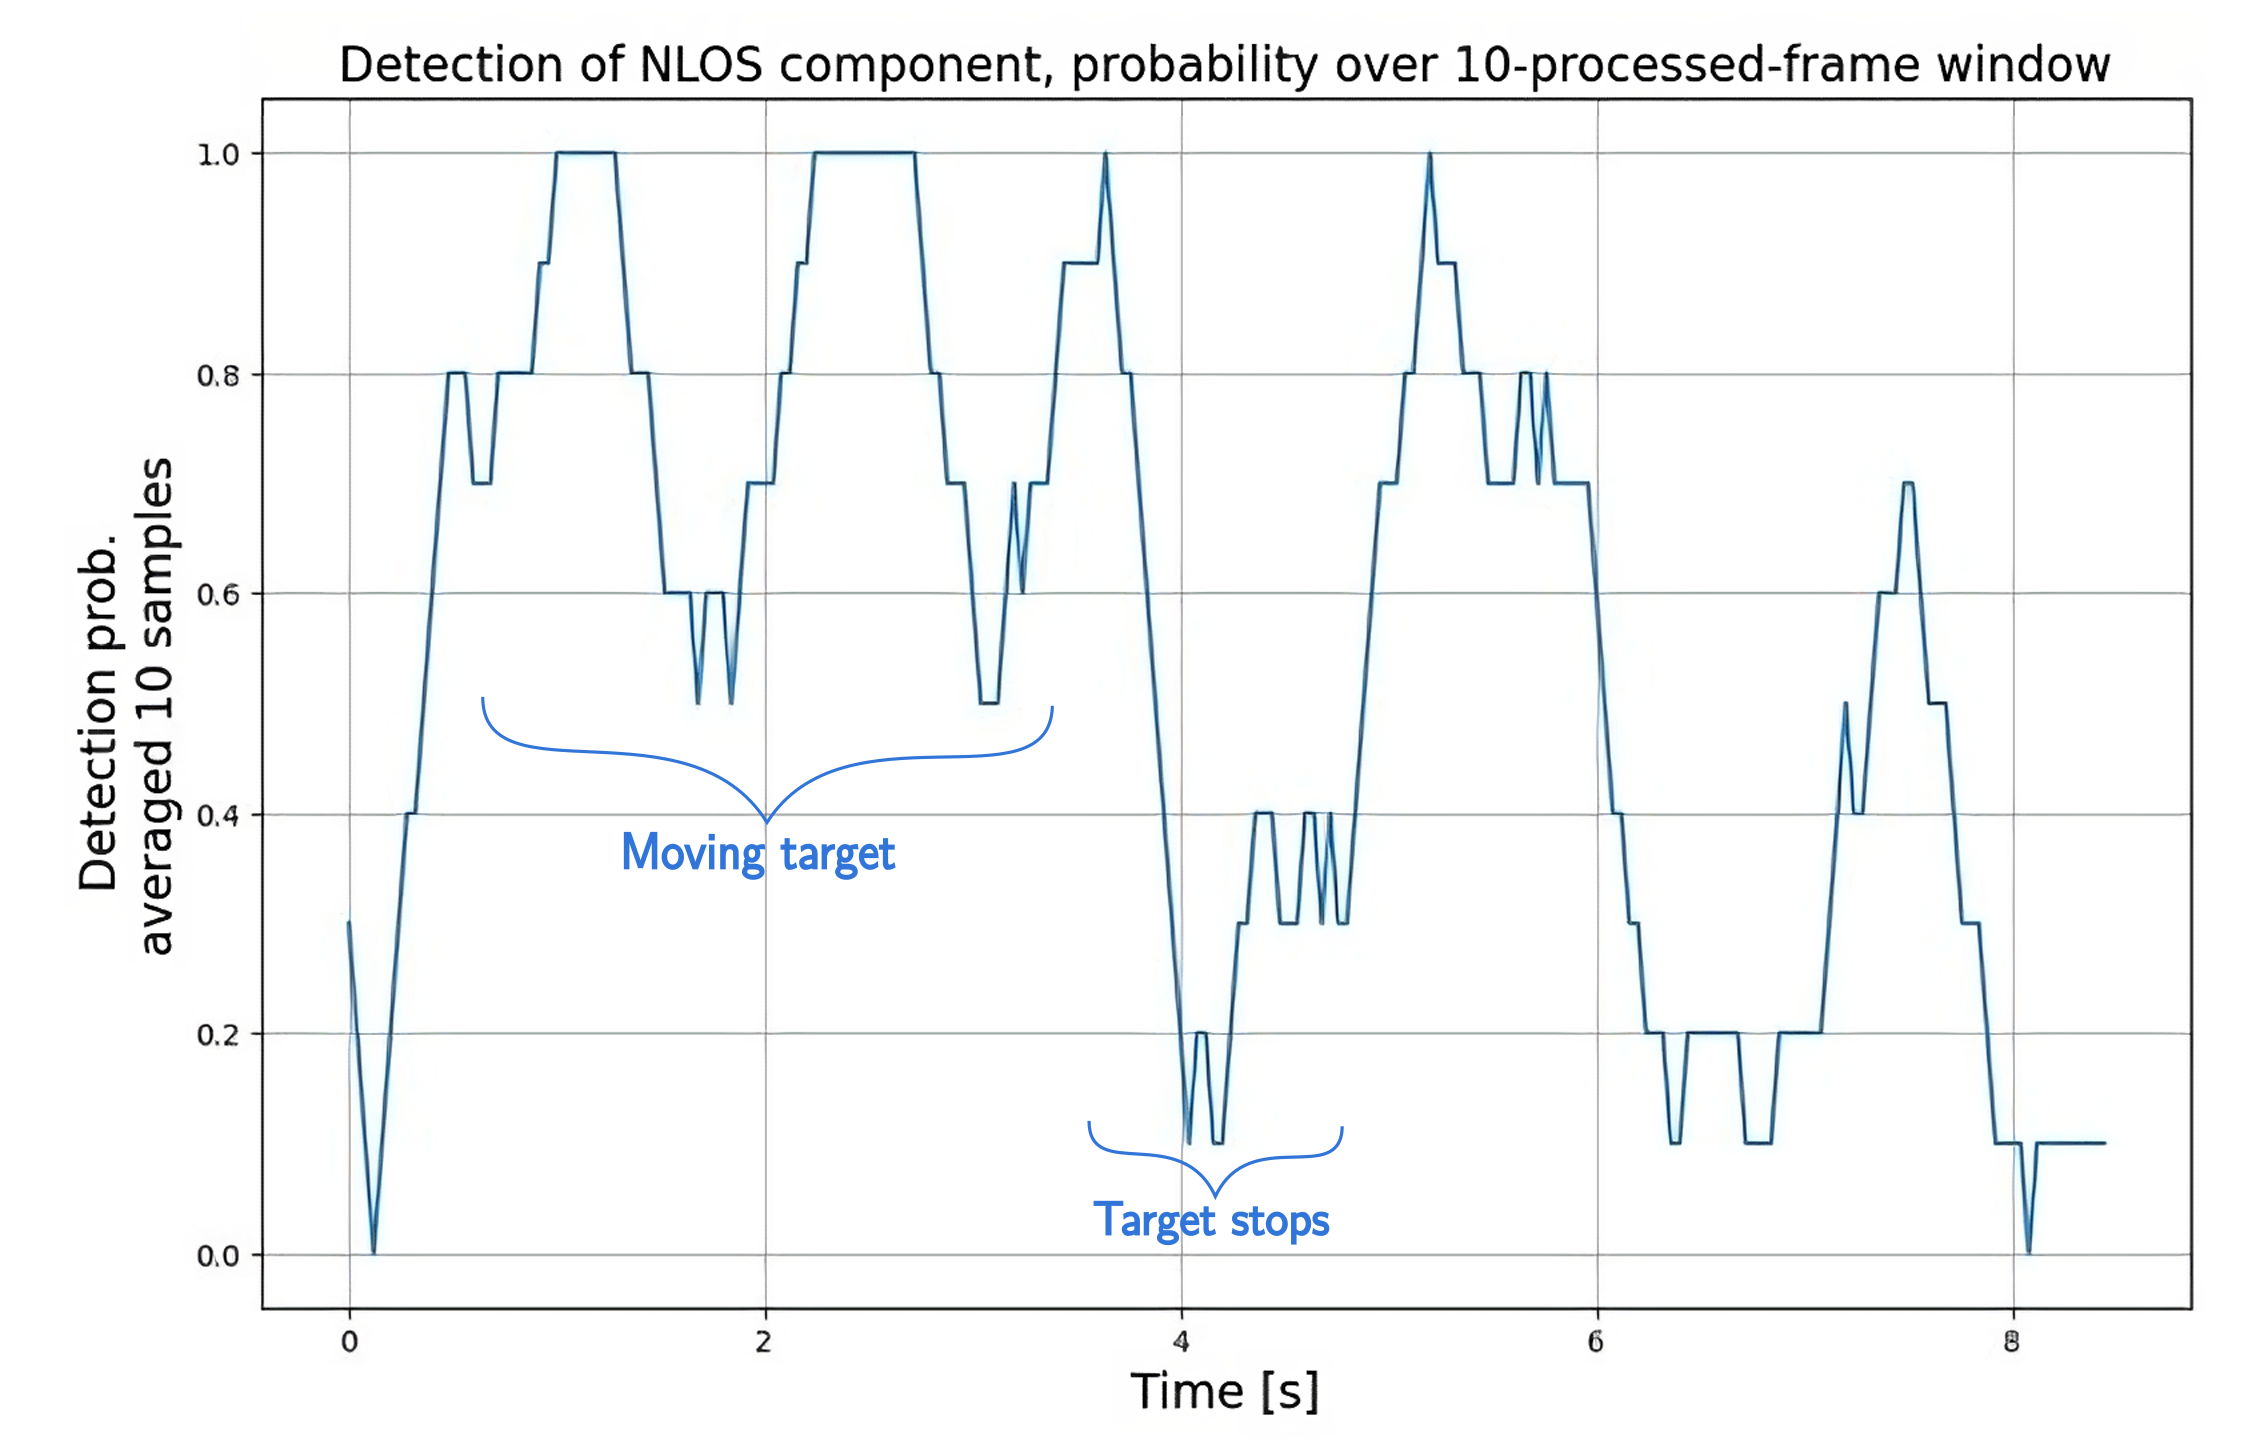
\includegraphics[width=0.7\textwidth]{Images/Test1/moving_avg-transformed_wtext}
	\caption{Detection rate observed for human target in mixed LOS/NLOS measurement.}
	\label{fig:Test1_moving_avg}
\end{figure}

\section{Observation on detection rate of a strong reflector}

The same measurement described in the previous section was repeated by moving the strong reflector described in \ref{sec:Test1_meas_scenario} in the same pattern as in the human case.

\begin{figure}[H]
	\centering
	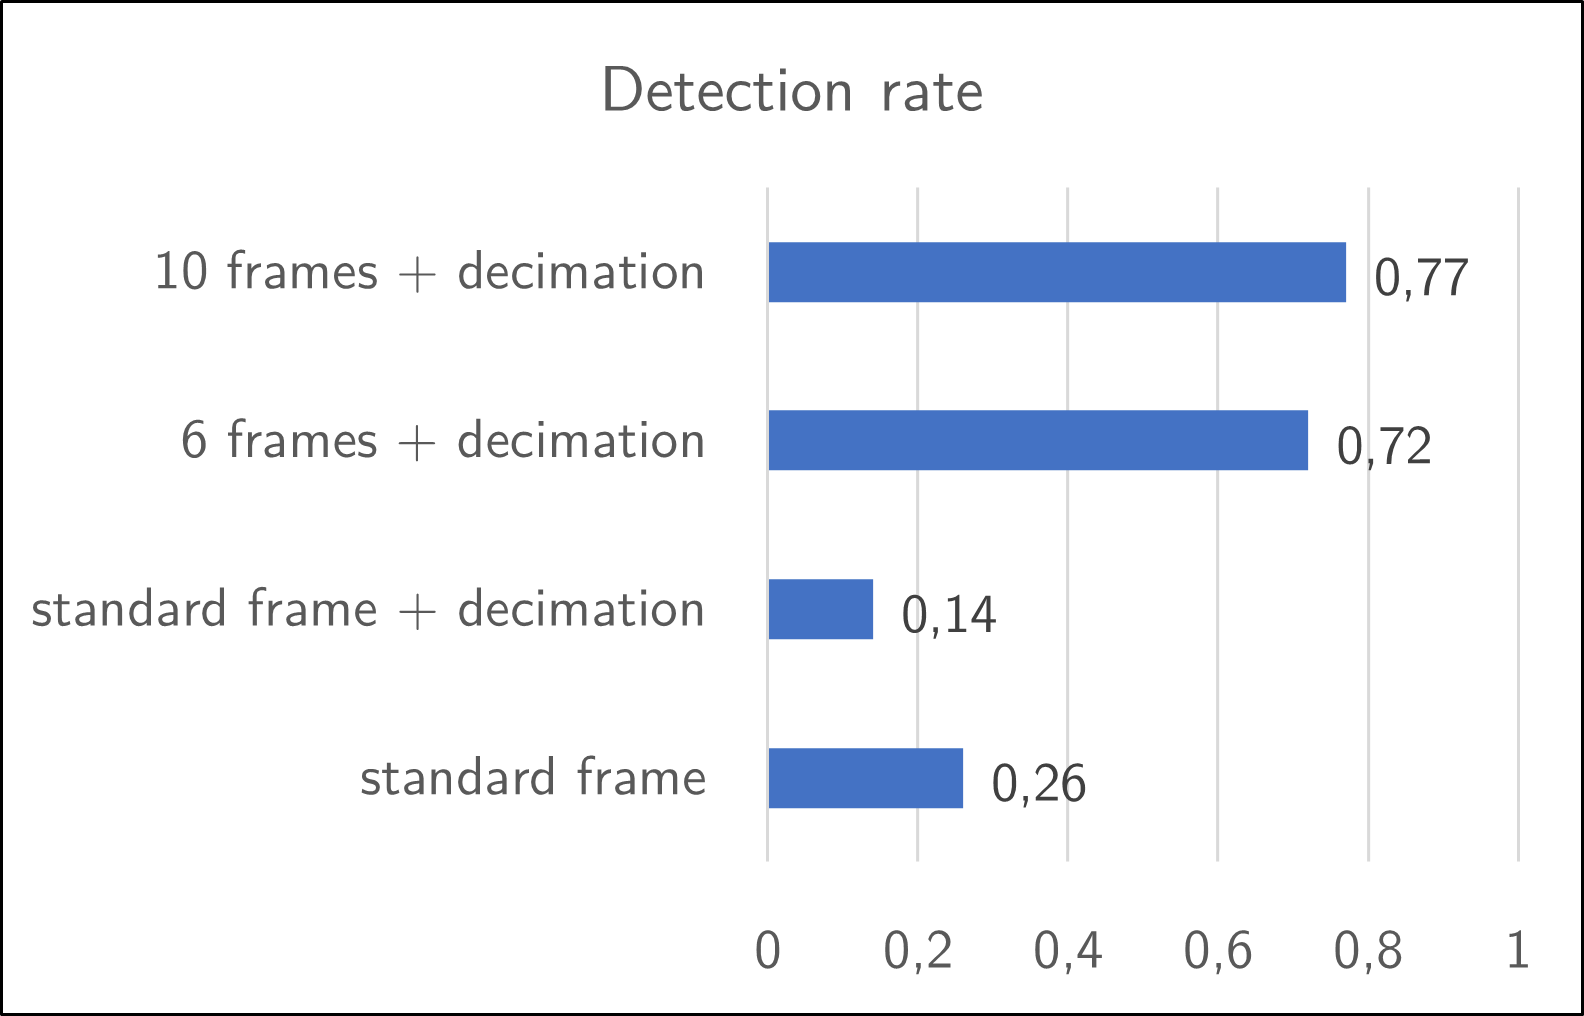
\includegraphics[width=0.7\textwidth]{Images/Test1/detect_hist_strong_ref.png}
	\caption{Detection rate observed for passive metal reflector target in mixed LOS/NLOS measurement.}
	\label{fig:Test1_detect_rate_strong_ref}
\end{figure}

The detection rate test displayed in figure \ref{fig:Test1_detect_rate_strong_ref} shows that the passive reflector, thanks to its significantly larger radar cross section, is clearly identified while it is moving and is not masked by clutter.

Passing the NLOS measurements to a Kalman filter it was possible to track the target in the range/Doppler plane, as shown in figure \ref{fig:Test1_kf_track_strong_ref}. This result is to show that one of the main limitation of NLOS signals is the strength of the target return. Objects with large RCS are easier to separate from the noisy background and the effect of fading and obstruction is relatively small.

\begin{figure}[H]
	\centering
	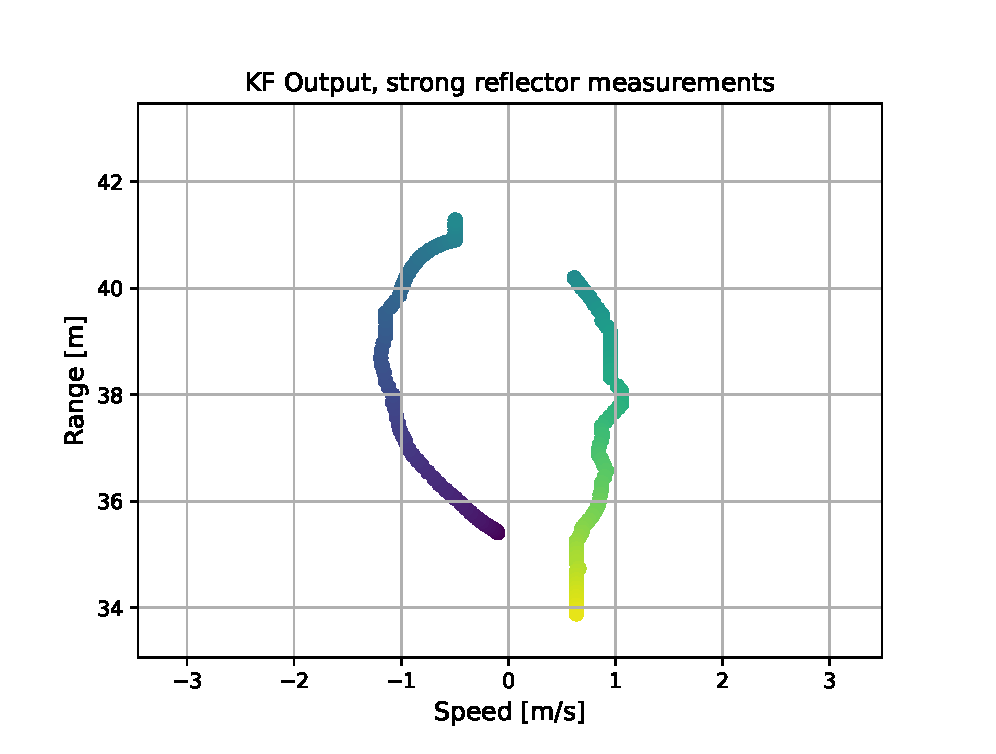
\includegraphics[width=0.7\textwidth]{Images/Test1/kf_track.eps}
	\caption{Output of KF tracking the target in the range/speed plane.}
	\label{fig:Test1_kf_track_strong_ref}
\end{figure}

